\documentclass[letterpaper, 12pt]{article}
\usepackage{tabularx} 
\usepackage{amsmath} 
\usepackage{graphicx} 
\usepackage{caption}
\captionsetup[figure]{font=footnotesize}
\usepackage[margin=1.1in,letterpaper]{geometry}
\usepackage{cite} 
\usepackage{textcomp}
\usepackage[final]{hyperref} 
\hypersetup{
	colorlinks=true,      
	linkcolor=blue,        
	citecolor=blue,        
	filecolor=magenta,     
	urlcolor=blue         
}
\usepackage{blindtext}



\begin{document}
	
	\title{CMLS Homework 2 - Distortion Effect Plugin}
	\author{E. Castelli, E. Intagliata, A. Rizzitiello, G. Zanocco}
	\date{May 2021}
	\maketitle
	
	\section{GitHub Repository}
	\url{https://github.com/ElisaCastelli/CMLS-HW2-Group11.git}
	
	\section{GUI}
	
	\begin{figure}[h!]
		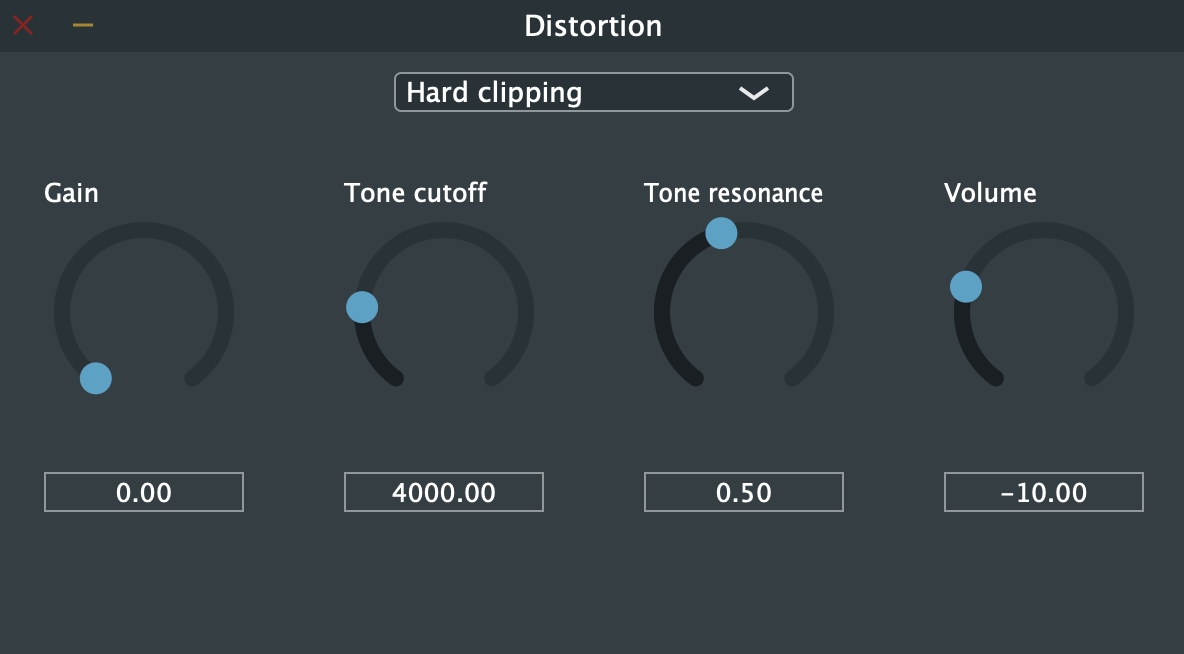
\includegraphics[scale=0.7]{gui.png}
		\centering
		\caption{Plugin's GUI}
		\label{fig:gui}
	\end{figure}

	Our plugin has been developed using a simple GUI, in Figure[\ref{fig:gui}], with the following graphic components:
	\\
	
	
	-	Gain knob 
	
	-	Tone cutoff knob 
	
	-	Tone resonance knob
	
	-	Volume knob
	
	-	Distortion type dropdown menu
	\\
	
	
	The gain knob is used to choose the level of the distortion effect applied to the sound, without affecting the output volume.
	The two tone knobs are used to control the brightness of the sound changing the parameters of a IIR low pass filter applied as last step of the computation. In particular with one knob we can control the cutoff frequency of the LPF and with the other we can control its resonance. 
	
	The volume knob allows the user to change the output amplitude of the sound.
	The dropdown menu is used to change the type of distortion effect applied to the sound. We have implemented five types of distortion: hard clipping, soft clipping exponential, soft clipping quadratic, soft clipping exponential, full wave rectification and half wave rectification.
	
	\section{Implementation}
	
	Our distortion plugin has been developed in C++, as programming language, using the JUCE cross-platform framework. We have followed a standard JUCE audio plugin development, implementing the two main classes Audio Processor and Audio Processor Editor. 
	Using this standard structure, we have been able to divide the more graphical part, implemented in the Audio Processor Editor class, from the one dedicated to audio processing, that is developed in the Audio Processor class.
	\\
	
	\textbf{-	Audio Processor Editor} 
\\
	
	In this class we have designed the Graphic User Interface by adding to the plugin window the graphic components we need: rotary sliders, in order to design the gain, tone and volume knobs, and a combo box menu, in Figure[\ref{fig:combobox}], in order to design the dropdown menu with which the user can choose the type of distortion effect to introduce.
	
	After having defined them, we have given to each element a fixed position and a size using the setBounds method.
	We haven’t redraw the style of the graphical elements with the LookAndFeel class but we have used the standard components.
	\\
	
	\begin{figure}[h!]
		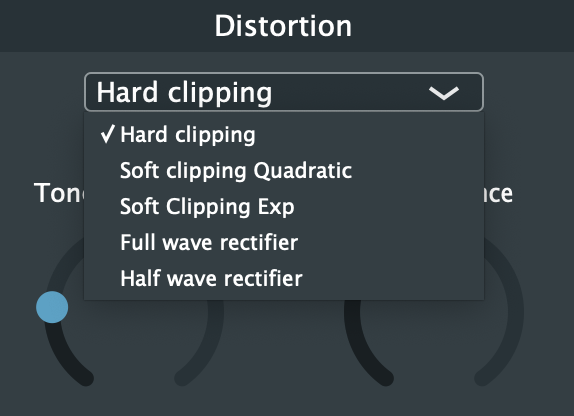
\includegraphics[scale=0.6]{combobox.png}
		\centering
		\caption{Dropdown menu}
		\label{fig:combobox}
	\end{figure}

	The connection between graphical elements and the Processor has been implemented using the AudioProcessorValueTreeState class. This method is an alternative to the Listener class, in order to connect each graphical component directly to a corresponding Audio Parameter.
	
	In particular, using  a SliderAttachment object for each Slider we have maintained a connection between the graphical Slider element and a parameter in AudioProcessorValueTreeState, keeping the two things in sync. We have used the same approach with a ComboBoxAttachment object to maintain the dropdown menu state.
	\\
	
	\textbf{-	Audio Processor 
}\\

        The processor contains the implementation of the distortion effect as well as the logic behind the different knobs.
        In its header file we defined some useful variables such as:
        
        \\
	-	oversampling: an object of class juce::dsp::Oversampling
	
	-	antiAliasingFilter: an IIR filter used in order to avoid aliasing after the oversampling
	
	-	toneFilter: an IIR tone-shaper filter
	
	-	lastSampleRate: sample rate of the input signal

	-	oversamplingFactor: the factor defining the oversampling step
        \\

        In the cpp file, specifically in the method processBlock, we used the method processSamplesUp in order to perform the oversampling of the input signal.
        Then we implemented the logic for the different distortion effects simply by applying 5 different non-linear functions to the oversampled signal.
        After that we took the distorted signal and filtered it with an anti-aliasing low-pass filter with cut-off frequency equal to the original sampling rate divided by 2.
        Finally we downsampled the signal down to the original sampling rate and applied anotherlow-pass filter with the purpose of shaping the sound of the distorted signal.  
	
	\begin{thebibliography}{99}
		
	\end{thebibliography}
	
	
\end{document}
